% Beamer
\PassOptionsToPackage{unicode}{hyperref}  % Evita errores con caracteres no ASCII
\PassOptionsToPackage{naturalnames}{hyperref} % tex.stackexchange.com/questions/10555
\documentclass[compress]{beamer}

% Idioma
\usepackage[spanish]{babel} % Traducciones
\usepackage[utf8]{inputenc} % Uso de caracteres UTF-8
\usepackage{lmodern}        % Fuentes de tamaño arbitrario
\usepackage[T1]{fontenc}    % Permite copiar y evita errores
\uselanguage{Spanish}       % Traducciones beamer
\languagepath{Spanish}      % (tex.stackexchange.com/questions/168208)

% Matemáticas
\usepackage{amsfonts}
\usepackage{amsmath}
\usepackage{amssymb}

% Colores
\definecolor{backg}{HTML}{F2F2F2}    % Fondo
\definecolor{title}{HTML}{bdc3d1}    % Títulos
\definecolor{comments}{HTML}{BDBDBD} % Comentarios
\definecolor{keywords}{HTML}{08388c} % Palabras clave
\definecolor{strings}{HTML}{FA5858}  % Strings
\definecolor{links}{HTML}{2C2C95}    % Enlaces
\definecolor{bars}{HTML}{045FB4}     % Barras (gráfico)


% Código
\usepackage{listings}
\lstset{
	language=[LaTeX]TeX,
	basicstyle=\footnotesize,
	morekeywords={href,uselanguage,languagepath,column},
	otherkeywords={pause,usetheme,usecolortheme,useinnertheme,titlepage,tableofcontents,subtitle},
	breaklines=true,
	backgroundcolor=\color{backg},
	keywordstyle=\color{keywords},
	commentstyle=\color{comments},
	stringstyle=\color{strings},
	tabsize=2,
	% Acentos, ñ, ¿, ¡ (tex.stackexchange.com/questions/24528)
	extendedchars=true,
	literate={á}{{\'a}}1 {é}{{\'e}}1 {í}{{\'i}}1 {ó}{{\'o}}1
	{ú}{{\'u}}1 {ñ}{{\~n}}1 {¡}{{\textexclamdown}}1
	{¿}{{?`}}1
}

% Gráficos
\usepackage{pgfplots}
\pgfplotsset{width=7cm,compat=1.8} % Opciones para gráficos

% Emoticonos
\usepackage{wasysym}

% tikz
\usepackage{tikz}
\usetikzlibrary{mindmap,trees,shadows}
\tikzset{ % Genera overlays
	invisible/.style={opacity=0},
	visible on/.style={alt={#1{}{invisible}}},
	alt/.code args={<#1>#2#3}{\alt<#1>{\pgfkeysalso{#2}}{\pgfkeysalso{#3}}},
}

%% Comandos %%
\newcommand{\ejemplo}[1]{\lstinputlisting{./examples/#1}} % Mostrar código de ejemplos
\newcommand{\muestra}[1]{\input{./examples/#1}}           % Mostrar ejemplos
\newcommand{\seccion}[1]{\input{./sections/#1}}           % Incluir secciones
\newcommand{\espacio}{\vspace*{\baselineskip}}            % Añade espacios
\newcommand{\beamer}{\texttt{beamer} }                    % Estilo único para beamer
\newcommand{\enlace}[3]{\href{#1}{\textbf{#2}} - {\small #3}}  % Estílo único para refs
\newcommand{\comando}[1]{{\color{black}\textbackslash}{\color{keywords}#1}}



\mode<presentation> {
	%\usetheme{default}
	%\usetheme{AnnArbor}
	%\usetheme{Antibes}
	%\usetheme{Bergen}
	%\usetheme{Berkeley}
	%\usetheme{Berlin}
	%\usetheme{Boadilla}
	%\usetheme{CambridgeUS}
	%\usetheme{Copenhagen}
	%\usetheme{Darmstadt}
	%\usetheme{Dresden}
	%\usetheme{Frankfurt}
	%\usetheme{Goettingen}
	%\usetheme{Hannover}
	%\usetheme{Ilmenau}
	%\usetheme{JuanLesPins}
	%\usetheme{Luebeck}
	\usetheme{Madrid}
	%\usetheme{Malmoe}
	%\usetheme{Marburg}
	%\usetheme{Montpellier}
	%\usetheme{PaloAlto}
	%\usetheme{Pittsburgh}
	%\usetheme{Rochester}
	%\usetheme{Singapore}
	%\usetheme{Szeged}
	%\usetheme{Warsaw}
	
	% As well as themes, the Beamer class has a number of color themes
	% for any slide theme. Uncomment each of these in turn to see how it
	% changes the colors of your current slide theme.
	
	%\usecolortheme{albatross}
	%\usecolortheme{beaver}
	%\usecolortheme{beetle}
	%\usecolortheme{crane}
	%\usecolortheme{dolphin}
	%\usecolortheme{dove}
	%\usecolortheme{fly}
	%\usecolortheme{lily}
	%\usecolortheme{orchid}
	%\usecolortheme{rose}
	%\usecolortheme{seagull}
	%\usecolortheme{seahorse}
	%\usecolortheme{whale}
	%\usecolortheme{wolverine}
	
	%\setbeamertemplate{footline} % To remove the footer line in all slides uncomment this line
	%\setbeamertemplate{footline}[page number] % To replace the footer line in all slides with a simple slide count uncomment this line
	
	%\setbeamertemplate{navigation symbols}{} % To remove the navigation symbols from the bottom of all slides uncomment this line
}

\usepackage{graphicx} % Allows including images
\usepackage{booktabs} % Allows the use of \toprule, \midrule and \bottomrule in tables



%% Título y otros %%
\title{Prácticas Fundamentos de Redes\\ Chat}
\author{Rubén Morales Pérez \\
	Francisco Javier Morales Pérez}
\date{\today}


%% Presentación %%
\begin{document}


\begin{frame}
\titlepage
\end{frame}

\begin{frame}{Índice}
  \hypertarget{index}{}
  \tableofcontents
\end{frame}


\section{Introducción}
\begin{frame}{Introducción}
	\begin{block}{Chat}
		En esta práctica crearemos un chat multiusuario usando el paradigma cliente-servidor. El servidor será
		un proceso alojado en alguno de los ordenadores de la comunicación.

		Usaremos como host la dirección IP local.
	\end{block}
	\begin{alertblock}{Cuidado}
		Hay redes wifi que bloquean ciertas comunicaciones, por eso
		hay que tener especial cuidado a la hora de ejecutar los programas.
	\end{alertblock}
\end{frame}


% -----------------------------------


\begin{frame}{Introducción}
	\begin{block}{Esquema}
		El esquema que usaremos será una clase \textit{Writer} y una clase \textit{Printer}, la primera se encargará de mandar los mensajes al servidor, la segunda de recibirlos y mostrarlos con el formato adecuado.
	\end{block}
\end{frame}


% -----------------------------------


\begin{frame}{Introducción}
	\begin{exampleblock}{Esquema}
		\begin{figure}[H]
    		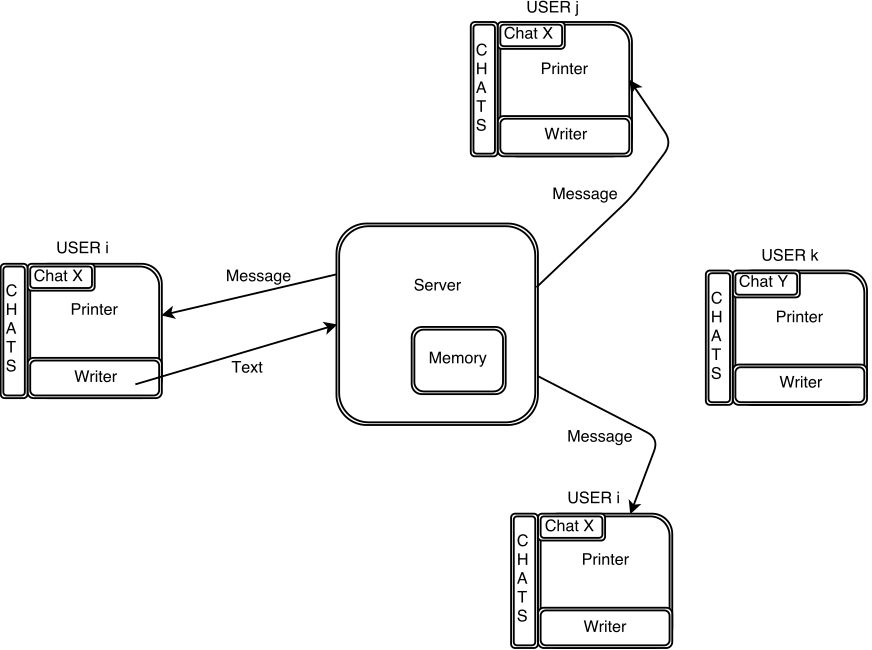
\includegraphics[scale=0.31]{./Imagenes/chat.png}
		\end{figure}
	\end{exampleblock}
\end{frame}

\section{Servidor}

\begin{frame}{Servidor}
	\begin{block}{Servidor}
		El servidor será una clase Server que estará continuamente recibiendo y mandando mensajes a los usuarios correspondientes. El servidor tiene una serie de archivos guardados para su organización.
	\end{block}
\end{frame}


% -----------------------------------


\begin{frame}{Servidor}
	\begin{exampleblock}{Esquema}
		\begin{figure}[H]
    		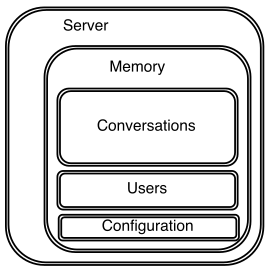
\includegraphics[scale=0.7]{./Imagenes/server.png}
		\end{figure}
	\end{exampleblock}
\end{frame}


\section{Usuario}
\subsection{Representación}

\begin{frame}{Usuario}
	\begin{block}{Representación}
		Un usuario quedará identificado por su idUser, los usuarios se guardarán en una carpeta especial con
		ficheros como el siguiente.
	\end{block}
	
	\begin{exampleblock}{0.usr}
	\begin{columns}
		\column	{.35\textwidth}
		\lstinputlisting{../.chatConfig/users/0.usr}
		
		\column	{.65\textwidth}
		\begin{itemize}
			\item Identificador de usuario
			\item Nombre de usuario
			\item Contraseña
			\item Grupos a los que pertenece
		\end{itemize}	
	\end{columns}
	\end{exampleblock}
\end{frame}


% -----------------------------------

\subsection{Conversaciones}
\begin{frame}{Conversaciones}
	\begin{block}{Mensajes}
	Los mensajes tienen un identificador del grupo al que pertenecen, del usuario que los envía y un iden-
	tificador del mensaje. Estos tres parámetros formarán la clave primaria, también se incluirá la fecha del envío del mensaje.
	\end{block}
	
	\begin{exampleblock}{ }
		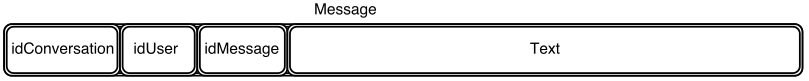
\includegraphics[scale=0.43]{./Imagenes/message.png}
	\end{exampleblock}
\end{frame}


% -----------------------------------


\begin{frame}{Fichero conversación}
	\begin{block}{ }
		Un fichero de conversación será una sucesión de mensajes.
	\end{block}
	
	\begin{exampleblock}{example.chat}
		\begin{figure}[H]
		\lstinputlisting{../.chatConfig/conversations/example.chat}
		\end{figure}
	\end{exampleblock}
\end{frame}


% -----------------------------------






\section{Configuración}
\begin{frame}{Configuración}
			El servidor alojará en ficheros las conversaciones, los usuarios y sus ajustes.
	\begin{block}{Clase Config}

		En la clase tendremos los
		directorios necesarios para guardar la información.
		
		Habrá variables para controlar los usuarios y conversaciones tenemos registrados en el sistema, los puertos usados para las comunicaciones y el host del servidor. 
	\end{block}
	
	\begin{block}{ }
		Guardadas las extensiones de los ficheros de usuarios y conversaciones. Desde el servidor podremos acceder al fichero de cada conversación o usuario.

		Debemos guardar la configuración al cerrar el servidor.

	\end{block}
\end{frame}


% -----------------------------------









\end{document}

